%% amssamp1.tex is nearly identical to amssamp2.tex, except
%% that amssamp2.tex uses the [twocol] option to produce
%% two-column text.

%\documentclass{ametsoc}
\documentclass{ametsoc}
\journal{jtech}

%\usepackage{amsmath}
\usepackage[draft]{hyperref}
\usepackage{color}

\usepackage{graphicx}
\graphicspath{{./fig/}}

%%%%%%%%%%%%%%%%%%%%%%%%%%%%%%%%
%Citations should be of the form ``author year''  not ``author, year''
\bibpunct{(}{)}{;}{a}{}{,}

\title{Turbulence Measurements from Compliant Moorings - Part II: Motion Correction}

\author{Levi F. Kilcher\correspondingauthor{Levi Kilcher, National Renewable Energy Laboratory, 15013 Denver West Pkwy, Golden, Colorado, USA}}

\affiliation{National Renewable Energy Laboratory, Golden, Colorado, USA}
\email{Levi.Kilcher@nrel.gov}

\extraauthor{Jim Thomson}
\extraaffil{Applied Physics Laboratory, University of Washington, Seattle, Washington, USA}

\extraauthor{Samuel Harding}
\extraaffil{Pacific Northwest National Laboratory, Richland, Washington, USA}

\extraauthor{Sven Nylund}
\extraaffil{Nortek AS, Norway}

\graphicspath{{./fig/}}
\newlength{\onewidth}
\setlength{\onewidth}{3.2in}

\newcommand{\note}[1]{\textcolor{blue}{#1}}
\newcommand{\citeneeded}[1]{\textcolor{red}{(NEED CITATION for: #1)}}
\usepackage{defs}

\abstract{
Acoustic Doppler velocimeters (ADVs) are a valuable tool for making high-precision measurements of turbulence, and moorings are a convenient and ubiquitous platform for making many kinds of measurements in the ocean. However---because of concerns that mooring motion can contaminate turbulence measurements and acoustic Doppler profilers are relatively easy to deploy---ADVs are not frequently deployed from moorings.  This work demonstrates that inertial motion measurements can be used to reduce motion-contamination from moored ADV velocity measurements. Three distinct mooring platforms were deployed in a tidal channel with inertial-motion-sensor-equipped ADVs. In each case, the motion correction based on the inertial measurements dramatically reduced contamination from mooring motion. The spectra from these measurements have a shape that is consistent with other measurements in tidal channels, and have a $f^{-5/3}$ slope at high frequencies---consistent with Kolmogorov's theory of isotropic turbulence. Motion correction also improves estimates of cross spectra and Reynold's stresses. Comparison of turbulence dissipation with flow speed and turbulence production indicates a bottom boundary layer production-dissipation balance during ebb and flood that is consistent with the strong tidal forcing at the site. These results indicate that inertial-motion-sensor-equipped ADVs are a valuable new tool for measuring turbulence from moorings.
}

\begin{document}

\maketitle


\section{Introduction}

Acoustic Doppler velocimeters (ADVs) have been used to make high-precision measurements of water velocity for over 20 years \cite[]{Kraus++1994, Lohrmann++1995}.  During that time, they have been deployed around the world to measure turbulence from a range of platforms, including stationary structures on ocean- and lake-bottoms, in surface waters from a pole lowered from a ship's bow, and in the deep ocean from autonomous underwater vehicles \cite[e.g.,][]{Voulgaris+Trowbridge1998, Zhang++2001, Kim++2000, Goodman++2006, Lorke2007, Geyer++2008, Cartwright++2009}. 

% \cite{Lueck++2002} has a good review of turbulence measurements. 

A relatively small fraction of ADV measurements have been made from moorings \cite[e.g.,][]{Fer+Paskyabi2014}. Presumably this is because mooring motion can contaminate ADV measurements, and acoustic Doppler profilers (ADPs) can be used to measure mid-depth turbulence statistics without a mooring \cite[e.g.,][]{Stacey++1999a, Rippeth++2002, Wiles++2006}. Still, ADV measurements have distinct characteristics that can be advantageous: they are capable of higher sample rates, have higher signal-to-noise ratios, and have a much smaller sample volume (1 centimeter, as opposed to several meters). That is, compared to an ADP, ADVs are high-precision instruments capable of providing unique information. They could be more widely used as a moored instrument (i.e., at an arbitrary depth) if a method for accounting for mooring motion can be demonstrated to provide more accurate estimates of turbulence statistics.

Inertial motion unit (IMU) sensors have been used in the aerospace and aeronautical industries to quantify the motion of a wide range of systems for several decades \cite[]{Bevly2004}. Over the last 10 years, the smartphone, drone, and `Internet of Things' markets has driven innovation in microelectrical-mechanical systems, including the IMU. As a result of this growth and innovation the cost, power requirements, and size of IMUs have come down. Also known as MARG (magnetic, angular-rate, gravity), or AHRS (attitude heading reference system) sensors, IMUs measure three axes of the Earth's magnetic field, angular rotation, and linear acceleration.\footnote{Within this literature, IMU is generally reserved for a MARG sensor without a magnetometer, but herein we refer to the entire group of sensors that measure motion using accelerometers and angular-rate sensors as IMUs.} These signals are then integrated using Kalman filters to estimate the orientation and motion of the sensor \cite[]{Barshan+Whyte1995, Marins++2001, Bachmann++2003}.

Nortek now offers a version of their Vector ADV with a Microstrain 3DM-GX3-25 IMU sensor \cite[]{vector_manual2005, MicroStrain2012a}. The IMU's signals are incorporated into the Vector data stream so that the motion and orientation signals are tightly synchronized with the ADV's velocity measurements. This tight synchronization provides a data stream that can be utilized to quantify ADV motion in the Earth's inertial reference frame, and remove that motion from the ADV's velocity measurements at each time step of its sampling. This work specifies a method for performing motion correction of these `ADV-IMU' measurements, and presents results of this method using data from a range of mooring configurations that positioned ADV-IMUs at mid-depths in Puget Sound. 

This effort was originally motivated by a need for low-cost, high-precision turbulence measurements for the emerging tidal energy industry \cite[]{Mccaffrey++2015, Alexander+Hamlington2015}. Experience in the wind energy industry has shown that wind turbine lifetime is reduced by atmospheric turbulence, and the same is expected to be true for tidal energy turbines. In wind, meteorological towers are often used to position sonic anemometers at the hub height of wind turbines for measuring detailed turbulence inflow statistics \cite[]{Hand++2003, Kelley++2005, Mucke++2011, Afgan++2013}. In the ocean, tower-mounted hub-height turbulence measurements have been made, but they are challenging to install and maintain in energetic tidal sites \cite[]{Gunawan++2014,Thomson++2012}. Therefore, the U.S. Department of Energy funded this work to investigate the accuracy of mooring-deployed ADV-IMUs to reduce the cost of turbulence measurements at tidal energy sites \cite[]{Kilcher++2016}. The approach proved to be successful and potentially useful to the broader oceanographic community interested in moored turbulence measurements \cite[]{Lueck+Huang1999, Doherty++1999, Nash++2004, Moum+Nash2009b, Alford2010, Paskyabi+Fer2013}.

The next section describes details of the measurements, including a summary of the hardware configurations (platforms) that were used to support and position the ADV-IMUs in the water column. A detailed description of the motion of these platforms is found in the companion paper to this work, \citeauthor{Harding++2017} (in review), hereafter Part 1. Section \ref{sec:methods} describes the mathematical details of motion correction and Section \ref{sec:results} presents results from applying the method to measurements from the various platforms. Section \ref{sec:discussion} is a discussion of the energetics of the tidal channel in which the measurements were made and demonstrates that the measurements are consistent with turbulence theory and other measurements in similar regimes. A summary and concluding remarks are provided in Section \ref{sec:conclusion}.


%%% Local Variables:
%%% mode: latex
%%% TeX-master: "Kilcher_etal_IMU-ADV"
%%% End:



\section{Measurements}
\label{sec:meas}

\begin{figure}[t]
  \centering
  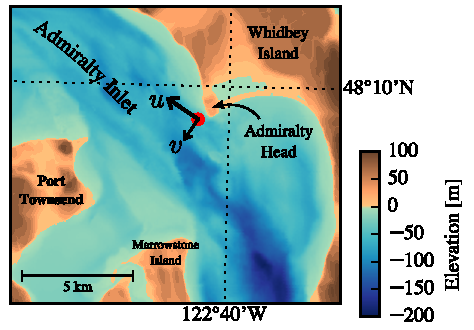
\includegraphics[width=3.4in]{map04_annot.pdf}
  \caption{Bathymetry of Admiralty Inlet near Port Townsend, Washington, U.S.A. \cite[]{Finlayson2005}. The red dot indicates the location of all measurements. The positive $u$ direction is the direction of ebb flow (thick arrow originating from red dot), and positive $v$ is away from Admiralty Head (smaller arrow).}
  \label{fig:map}
\end{figure}

This work focuses on measuring turbulence from ADVs that are deployed from nonstationary platforms and equipped with IMUs. The ADVs utilized for these measurements were equipped with Microstrain 3DM-GX3-25 IMU sensors that captured all six components of the ADV motion (three components of angular rotation and three components of linear acceleration), as well as the orientation of the ADV pressure case. The sampling of the motion sensor is tightly synchronized with the ADV measurements. The IMU measures its motion at 1 kHz and uses internal signal integration (Kalman filtering) to output the motion signals at the same sample rate as the ADV's velocity measurements. This reduces aliasing of the IMU's motion measurements above the ADV's sample rate \cite[]{3DM-GX3_coning_sculling}. Cable-head ADVs were used throughout this work to allow for flexibility in the positioning of the ADV head relative to its pressure case.

All measurements used in this work were made in Admiralty Inlet, Washington, approximately 500 m west southwest of Admiralty Head in 60-m of water near 48\deg\ 9.18' N, 122\deg\ 41.22' W (Figure \ref{fig:map}). The site is approximately 6 km east of Port Townsend, and 1 km north of the Port Townsend to Coupeville ferry route.  Admiralty inlet is the largest waterway connecting Puget Sound to the Strait of Juan de Fuca, and it possesses a large semidiurnal tidal flow \cite[]{Thomson++2012, Polagye+Thomson2013}.  This work utilizes data from three distinct deployment platforms: the tidal turbulence mooring, a StableMoor buoy, and a simple sounding weight.  All data used in this analysis is available from the MHK data repository (http://mhkdr.openei.org; submission ids: 49, 50 and 51). Additional details, photos, and schematic diagrams of all three mooring systems can be found in Part 1.

\subsection{Tidal Turbulence Mooring}

The tidal turbulence mooring (TTM) is a simple mooring system with a strongback fin suspended between a steel clump-weight anchor weighing 1,200 kg when dry and a 0.93-m-diameter spherical steel buoy with a buoyancy of 320 kg. The ADV pressure cases were clamped to one side of the strongback fin and the ADV sensor head was positioned 10 cm in front of the fin's leading edge (Figure \ref{fig:ttm:diagram}). The leading edge of the fin is fastened inline with the mooring line. This configuration  was designed to work like a weather vane, such that the drag on the fin held the ADV head upstream of the mooring components.  This work utilizes data from two TTM deployments. 

\subsubsection{June 2012 TTM deployment}

The first TTM deployment was in June 2012 from 17:30 on the 12th until 14:30 on the 14th (local; i.e., Pacific Daylight Time). Two Nortek ADVs were clamped to either side of the fin so that the axis of their cylindrical pressure cases were parallel with the leading edge of the strongback. The ADV heads were spaced 0.5 m apart vertically along the fin. Only one of these ADVs was equipped with an integrated IMU. This TTM also had an upward-looking acoustic Doppler profiler mounted on the mooring anchor.

Periods of time during which this mooring interfered with a beam of the Doppler profiler were identified by inspecting the profiler's acoustic amplitude signal. Periods during which one beam of the profiler had $>5\%$ higher acoustic amplitude than the other beams were flagged as ``contaminated" and excluded from averaging.  Five-minute averages in which more than 50\% of the data were contaminated in this way were masked as invalid.

\subsubsection{June 2014 TTM deployment}

The second TTM deployment was in 2014 from 06:00 on June 17 to 05:00 on June 19 (local time).  Two Nortek ADV-IMUs were mounted on this TTM, with their heads spaced 0.5 m apart along the fin. In this case, the pressure cases and ADV heads were inclined at an angle of 18$^\circ$ to the leading edge of the fin to account for mooring blowdown during strong currents (Figure \ref{fig:ttm:photo}). This change was made to reduce vibrational motion observed during the June 2012 deployment that was believed to be associated with the orientation of the pressure cases.

\begin{figure}[t]
  \centering
  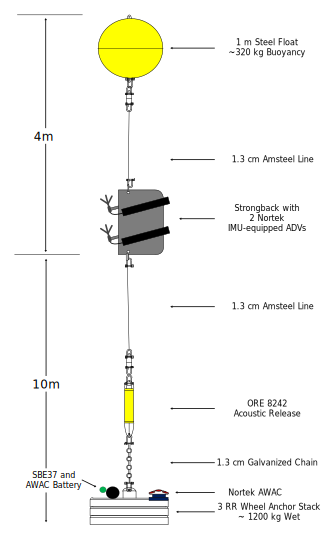
\includegraphics[width=2.4in]{TTM04b}
  \caption{Schematic diagram of the TTM; not to scale.}
  \label{fig:ttm:diagram}
\end{figure}

\begin{figure}[t]
  \centering
  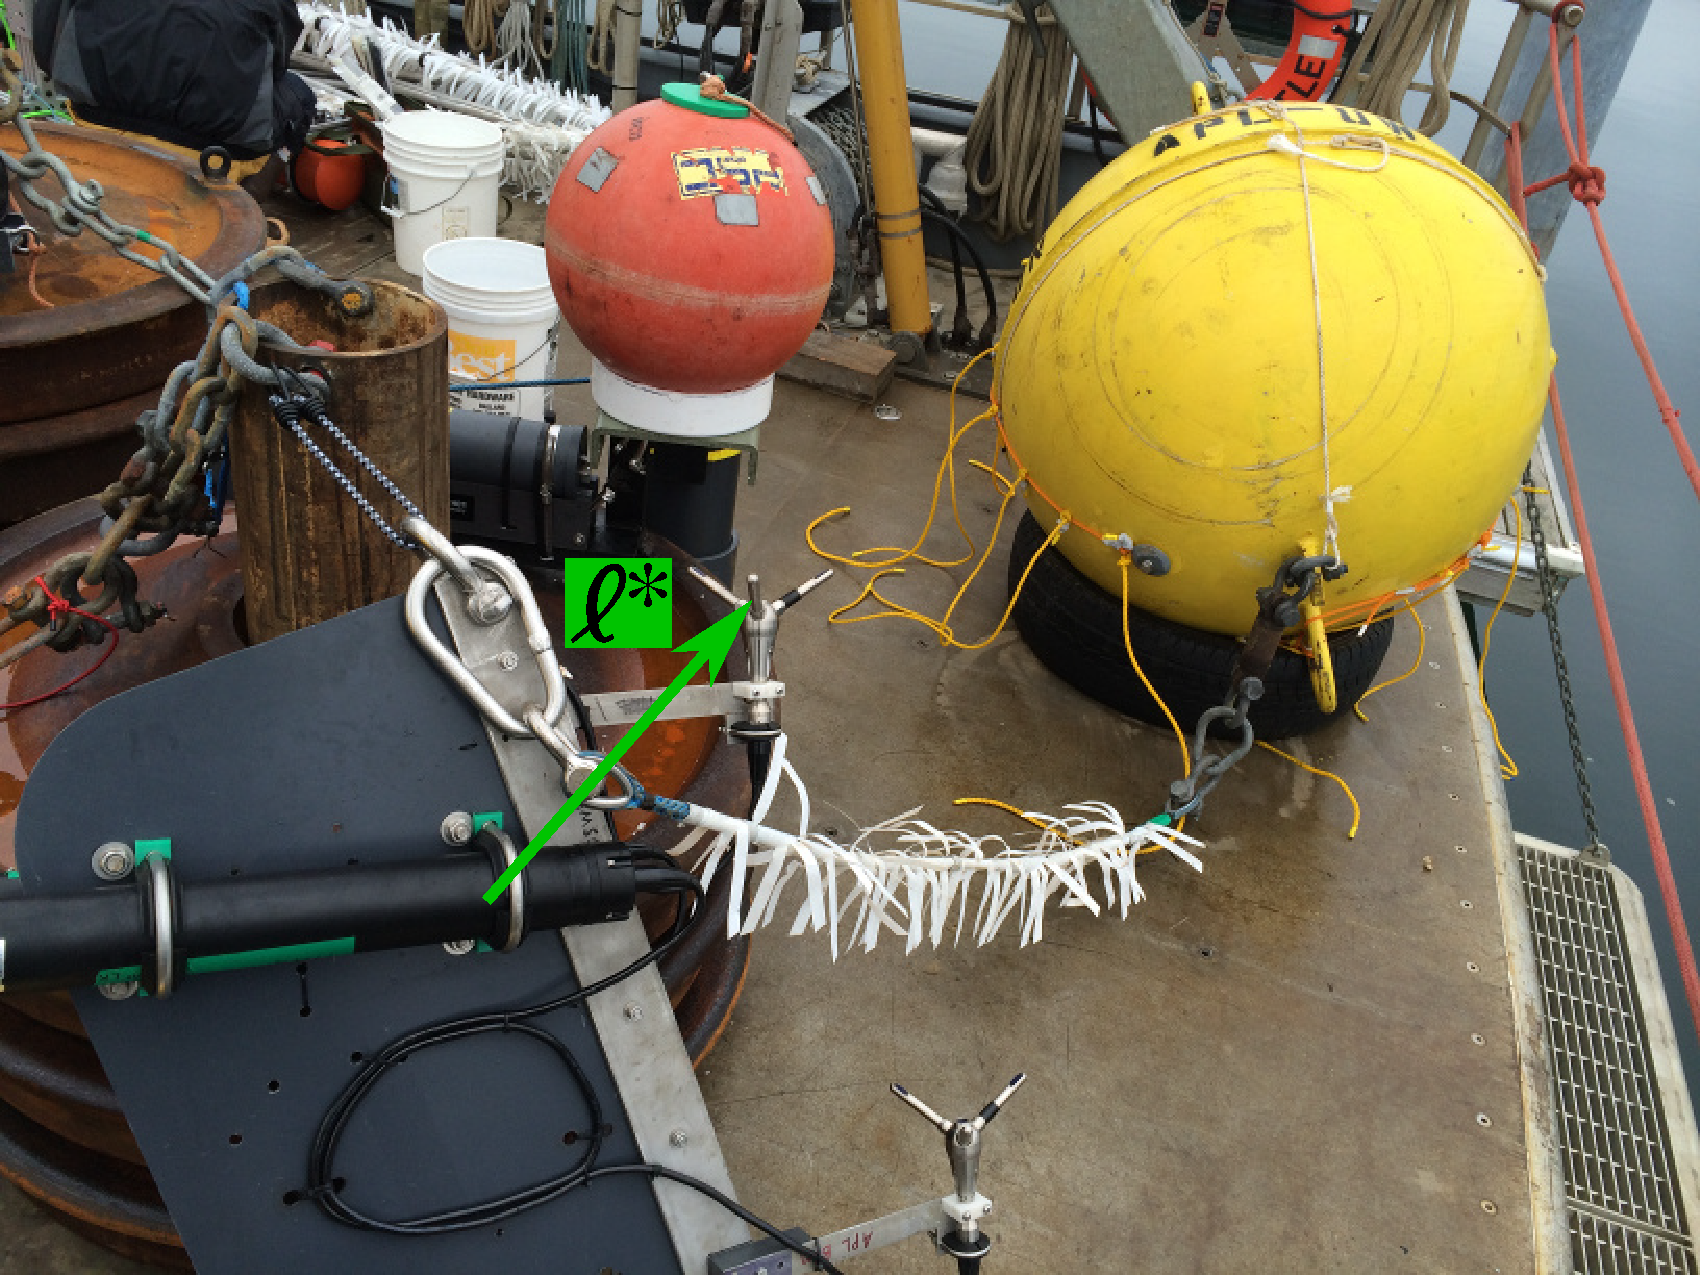
\includegraphics[width=2.6in]{TTM_image01_annot}
  \caption{TTM components on the deck of the R/V Jack Robertson. The TTM includes two ADVs, with pressure cases mounted on opposite sides of the fin. The anchor stack includes a pop-up buoy for retrieval. The green arrow indicates the vector from the IMU to the ADV head (face of the transmit transducer). }
  \label{fig:ttm:photo}
\end{figure}

\subsection{The StableMoor platform}

The second deployment platform was a cylindrical, StableMoor, syntactic foam buoy (manufacturer: Deep Water Buoyancy) that was anchored to a clump weight that weighed 2,700 lbs (Figure \ref{fig:SM}). The buoy is 3.5 m long and 0.45 m in diameter with a tail ring that is 0.76 m in diameter. The StableMoor buoy weighs 295 kg in air, and has a buoyancy of 185 kg in water. 

The StableMoor buoy was deployed with an ADV-IMU mounted at its nose from 11:21 on May 12 to 11:53 on May 13, 2015 (local time). The sample volume of the ADV is 10 cm forward of the nose and 20 cm above the center line of the StableMoor buoy (Figure \ref{fig:SM}). Based on \citeauthor{Wyngaard++1985}'s (1985) investigation of a similarly shaped slender body, the velocity measurements should have flow-distortion effects of less than 10\%. This configuration was designed to be the most stable platform for measuring turbulence from a moving platform. The StableMoor buoy was equipped with a 1,200-kHz RDI workhorse sentinel acoustic Doppler profiler that was oriented downward-looking to measure water velocity below the platform in twelve 1-m bins and measure buoy motion (``bottom tracking"), all at a 1-Hz sample rate. 

The buoy was ballasted to pitch upward a few degrees in zero-flow to avoid ``flying downward." In the presence of an oncoming current, the tail fins help to orient it into the flow. The anchor for this buoy is similar to that of the TTM, including an acoustic release so the mooring and anchor can be recovered separately.

The StableMoor platform has two primary advantages compared to the TTM. First, it is significantly more massive and hydrodynamically stable than the TTM, which reduces the frequency of motions of the platform. Second, the StableMoor platform is capable of supporting a bottom-tracking acoustic Doppler profiler, which provides an independent measure of the platform's translational motion. Disadvantages of the StableMoor include: its size, which adds to the challenge of deployment and recovery, and its cost, which is significantly higher than the TTM system.

\begin{figure}[t]
  \centering
  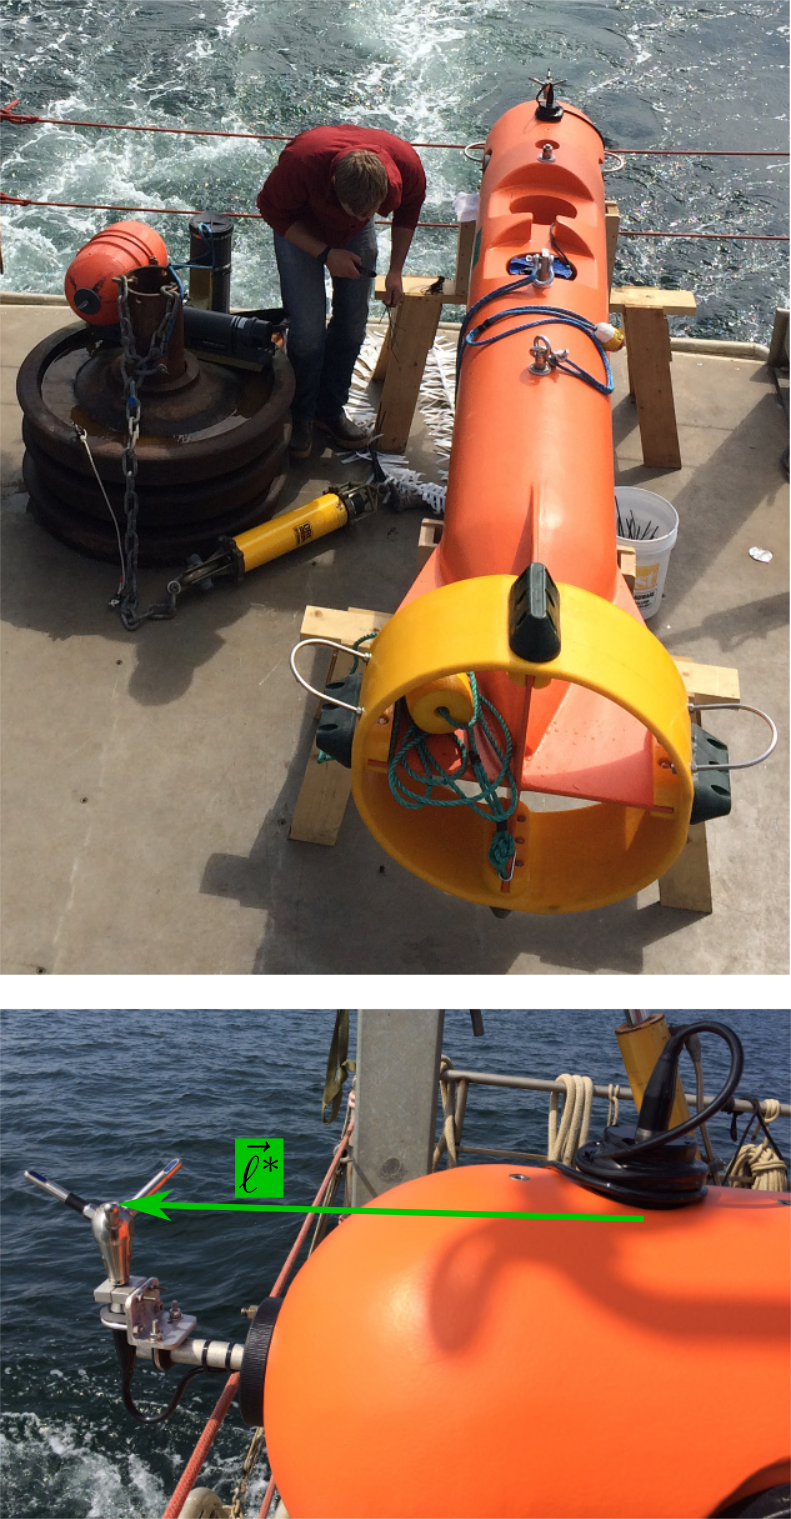
\includegraphics[width=2.6in]{StableMoor_Composite}
  \caption{Top: Alex DeKlerk checks to ensure that the StableMoor buoy is properly fastened to its anchor; the RDI workhorse ADCP can be seen in the rear instrument bay. A bridle is draped across the top of the buoy for deployment and recovery, and a small marker buoy fastened to the tail is useful during recovery.  Bottom: a close-up of the StableMoor with the ADV head and the top of its pressure case. The green arrow indicates the vector from the IMU to the ADV head. 
%Bottom: the StableMoor buoy in `wing mode', floating on the ocean surface with the marker buoy trailing behind. The ADV heads mounted at the ends of the cross-beam are protruding above the waterline.   
}
  \label{fig:SM}
\end{figure}

\subsection{Turbulence Torpedo}

The turbulence torpedo is a simple sounding weight with an ADV head mounted forward of the nose, and the ADV pressure case strapped below. This platform was deployed on May 14, 2015, for 37 minutes starting at 07:41 local time.  This measurement was made from a davit that hung the system from the side of the ship to a depth of approximately 25 m. The primary logistical advantages of this platform are its compact size, low cost, and the flexibility to perform spatial transects.  

\begin{figure}[th]
  \centering
  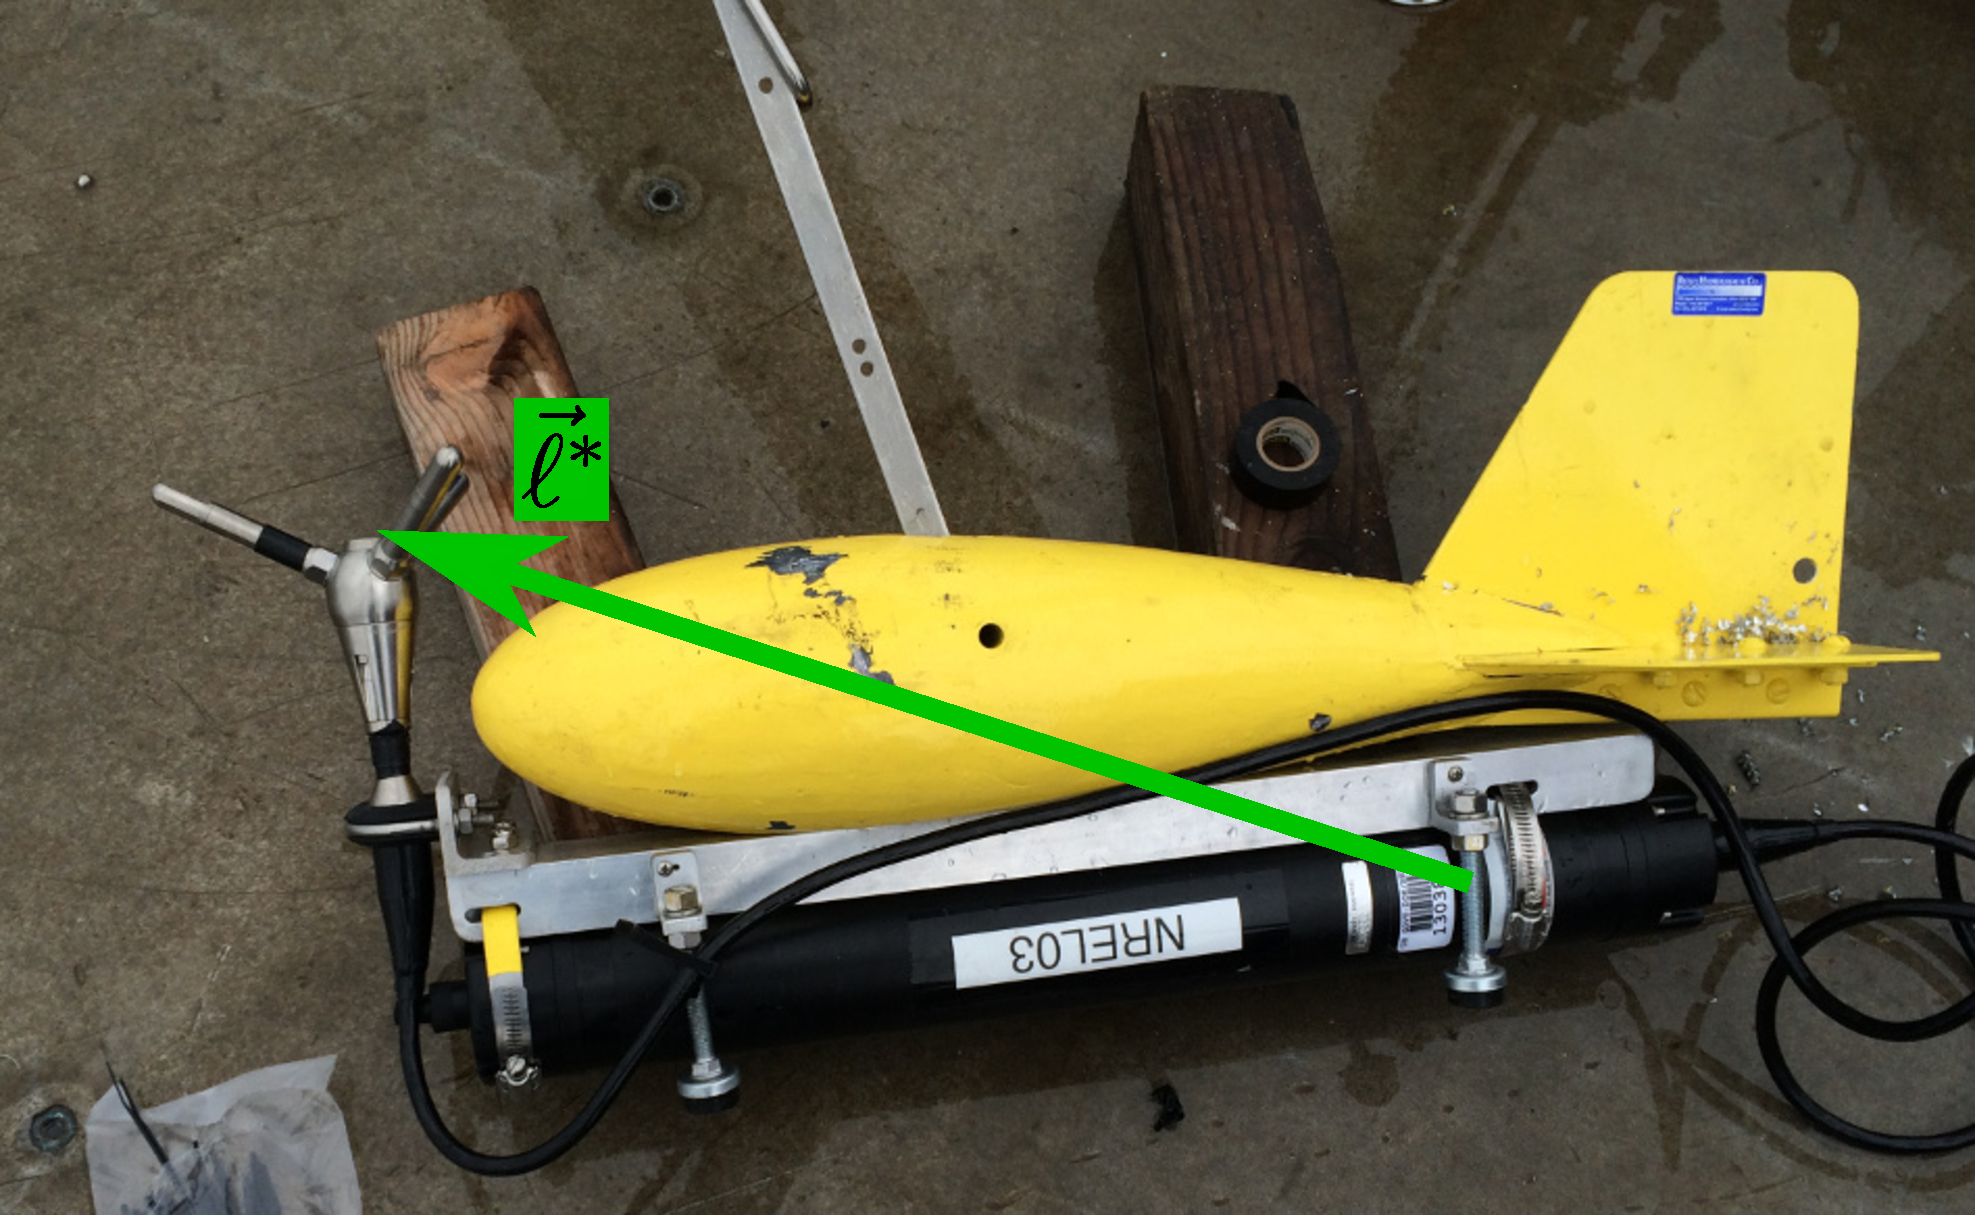
\includegraphics[width=2.6in]{Torpedo_Image01_annot}
  \caption{The turbulence platform showing details of the ADV head and pressure case configuration. The green arrow indicates the vector from the IMU to the ADV head. The head cable was taped out of the way beneath the sounding weight tail fins shortly after taking this photo.}
  \label{fig:torpedo}
\end{figure}

\subsection{Coordinate system and turbulence averaging}

Unless stated otherwise, vector quantities in this work are in a fixed ``principal-axes" coordinate system that is aligned with the bidirectional tidal flow: positive $u$ is in the direction of ebb (310$^\circ$ True), positive $w$ is vertically upward, and $v$ is the cross-stream component in a right-handed coordinate system. The full velocity vector, $\vec{\tilde{u}} = (\tilde{u}, \tilde{v}, \tilde{w})$, is separated into a mean and turbulent component as $\vec{\tilde{u}} = \vec{\bar{u}} + \vec{u}$, where the over-bar denotes a 5-minute average. Turbulence kinetic energy, $\tke = \uu + \vv+\ww$, and Reynold's stresses, $\uv$, $\uw$, $\vw$, are computed by averaging over the 5-minute window.  Throughout this work, we use $\bar{U} = (\bar{u}^2+\bar{v}^2)^{1/2}$ to denote the mean horizontal velocity magnitude. 

All spectra, $\spec{x}(f)=|\fourier{x(t)}|^2$, and cross spectra, $\cspec{x}{y}(f)=\mathrm{real}(\fourier{x(t)}\fourier{y(t)})$, are computed using NumPy fast Fourier transform routines \cite[]{Walt++2011}. Here, $\fourier{x(t)}$ denotes the fast Fourier transform of a signal $x(t)$. Time series, e.g., $x(t)$, are linearly detrended and Hanning windowed prior to computing $\fourier{x}$ to reduce spectral reddening.  

Throughout the remainder of this work, the dependence of $S$ and $C$ on $f$ is implied (e.g., $\spec{x}(f)$ is hereafter $\spec{x}$), and for other variables the dependence on $t$ is implied. Spectra and cross spectra are normalized to preserve variance: $\int \spec{u}\mathrm{d}f = \uu$, and  $\int \cspec{u}{v}\mathrm{d}f = \uv$. The notations $\spec{\ue}=(\spec{u}, \spec{v}, \spec{w})$, and $C\{\ue\} = (\cspec{u}{v}, \cspec{u}{w}, \cspec{v}{w} )$ denote the set of spectra and cross spectra for each velocity component and pairs of components, respectively.

Turbulence dissipation rates are computed as:
\begin{align}
  \epsilon = \frac{1}{\bar{U}}\left(\alpha\left\langle(\spec{u}+\spec{v}+\spec{w})f^{5/3}\right\rangle_{f_{IS}}\right)^{3/2}
\end{align}
Where  $\alpha=0.5$, and $\langle\rangle_{f_{IS}}$ denotes an average over the inertial subrange of the velocity spectra and where the signal-to-noise ratio is small \cite[]{Lumley+Terray1983,Sreenivasan1995}. Throughout this work, we take this average from 0.3 to 1 Hz for the $u$ and $v$ components, and 0.3 to 3 Hz for the $w$ component.

%%% Local Variables:
%%% mode: latex
%%% TeX-master: "Kilcher_etal_IMU-ADV"
%%% End:



\section{Methodology}
\label{sec:methods}


\def\ue{\ensuremath{\vec{\tilde{u}}\earth}}
\def\nrot{\ensuremath{\vec{n}_{\omega}}}
\def\nacc{\ensuremath{\vec{n}_{a}}}


This work describes a method for correcting velocity measurements from a moving velocity sensor, $\umeas$, using independent measurements of that sensor's motion, $\uhead$, to remove the motion from the velocity measurements, and thus estimate the `motion corrected velocity':
\begin{align}
  \label{eqn:u_mot_def}
  \ue(t) & = \umeas(t) + \uhead(t) \qquad .
\end{align}
Note here that the `+'-sign is correct because head motion, $\uhead$, induces a measured velocity in the opposite direction of the head motion itself ($\umeas = \ue - \uhead$). This approach has been used to successfully correct sonic anemometer measurements of atmospheric turbulence \cite[e.g., ][]{Edson++1998, Miller++2008}.  In the ocean, previous works have utilized inertial motion sensors to quantify the motion of multiscale profilers for the purpose of measuring the full spectrum of oceanic shear \cite[]{Winkel++1996}, and to quantify the motion of thermistor sensors \cite[]{Moum+Nash2009b}, but the \cite{Edson++1998} approach has not been documented for moored ADV measurements.

The Microstrain IMU available in the Nortek Vector ADV measures the linear acceleration, $\Accel$, rotational motion, $\AngRt$, and orientation matrix, $\omat$, of the ADV pressure case in the Earth reference frame at every time step of the ADV's sampling. So long as the ADV head is rigidly connected to the IMU (i.e. the ADV pressure case), the motion of the ADV head is calculated from these signals as the sum of rotational and translational motion:
\begin{align}
  \label{eqn:uhead}
\begin{split}
  \uhead & = \urot + \uacc + \ulow \\
      & = \omatinv \cdot \AngRt^*(t)\times\l + \int \rangle \Accel(t)\langle_{f_{a}} \,\mathrm{d}t + \ulow
\end{split}
\end{align}
Here, $*$ superscripts denote quantities in the ADV's local coordinate system, and $\l$ is the vector from the IMU to the ADV head. $\omatinv$---the inverse of the orientation matrix---rotates vectors from the IMU to the Earth reference frame. The notation $\rangle \cdot \langle _{f_a}$ indicates a high-pass filtering operation at frequency $f_a$. The high-pass filter reduces low-frequency noise in $\Accel$---sometimes referred to as bias drift---that is amplified by integration \cite[]{Barshan+Whyte1995, Bevly2004, Gulmammadov2009}. $\ulow$ is the low-frequency translational motion that is unresolved by $\uacc$, and it is discussed in more detail below. Note that, to avoid double counting, $\ulow$ should be estimated by applying the complementary low-pass filter to the independent measurement of low-frequency motion. We use fourth order, zero-phase (bidirectional), Hanning filters for all filtering operations.

\begin{figure}
  \centering
  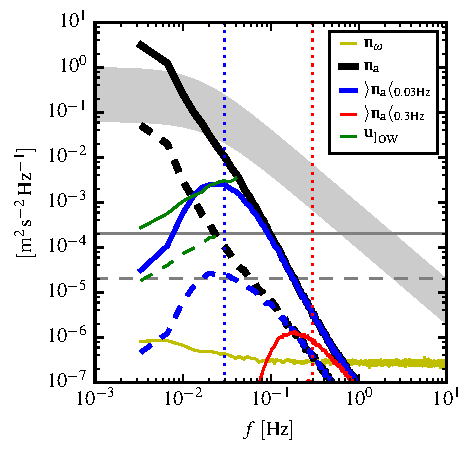
\includegraphics[width=\onewidth]{stationary_noise04}
  \caption{The spectral noise levels of rotational velocity ($\spec{\nrot}$, yellow) and translational velocity ($\spec{\nacc}$, black) estimated from an ADV-IMU resting motionless on a table. Solid and dashed lines indicate the horizontal and vertical components, respectively, of $\spec{\nacc}$ and $\spec{\ulow}$. The horizontal components are equivalent, as are all three components of $\spec{\nrot}$. The $\nacc$ signals are unfiltered (black), and high-pass filtered at 0.03 Hz (blue) and 0.3 Hz (red); vertical dotted lines indicate the filter frequency.  Green lines are an estimate of $\ulow$ for the TTM. Grey horizontal lines indicate the horizontal (solid) and vertical (dashed) Doppler noise levels of the ADV. The shaded region indicates the range of $u$ spectral amplitudes presented herein (0.002 $< \tke <$ 0.03 $\mathrm{m^2/s^2}$, 1e-5 $< \epsilon <$ 5e-4 $\mathrm{W/kg}$).}
  \label{fig:stnoise}
\end{figure}

The noise levels of the IMU, $\nrot$ and $\nacc$, are computed from ADV-IMU data collected while the instrument was resting motionless on a table for several hours. Where, for this motionless dataset, the noise levels are defined according to \eqref{eqn:uhead} with $\nrot$ in place of $\urot$, and $\nacc$ in place of $\uacc$.  These are presented in Figure \ref{fig:stnoise} relative to the ADV spectra presented in following sections of this paper (grey shading), and relative to the Doppler noise levels of the ADV.

$\spec{\nrot}$ is equal in all three components, and so only one component is presented for simplicity (yellow). $\spec{\nrot}$ is several orders of magnitude lower than the velocity spectra we measured (grey region), and also more than an order of magnitude smaller than the Doppler noise levels of the ADV. Here we have used $\l=1$ m; which is the order-of-magnitude of the typical distance between the ADV head and the IMU. This indicates that the precision of $\urot$ (i.e. the angular rate sensor) is adequate for making corrections to ADV velocity measurements without filtering.

The noise level of $\spec{\uacc}$ (Figure \ref{fig:stnoise}, black), on the other hand, is dominated by a $f^{-2}$ slope that results from integrating the low-frequency noise in $\Accel$. The horizontal ($u$ and $v$) spectra of these noise levels are identical, and so we only present one of them for simplicity (solid lines). The vertical spectra noise levels are different because the signal-to-noise ratio is larger (dashed black lines). High-pass filtering reduces the low-frequency noise (blue and red) so that it does not contaminate motion correction, but any real motion that does exist at these frequencies is lost \cite[]{EgelandPhD2014, VanZwieten++2015}. This means there is a residual low-frequency translational motion, $\ulow$, that needs to be measured independently---or at the very least considered---when using ADV-IMU data from moving platforms. 

%\def\ulow{\ensuremath{\vec{u}_{\textnormal{low-SMB}}}}
For the StableMoor buoy, the ADP bottom-track measured $\ulow$, and this measurement agrees with $\uacc$ over a narrow frequency band (see Part I, appendix A), indicating that the ADP and IMU are resolving the same motion. When this is the case, it is trivial to select a frequency in the middle of the spectral overlap (in this case, we choose $f_a=0.2$ Hz), and high-pass and low-pass filter $\uacc$ and $\ulow$, respectively, then sum to estimate total translational motion. This process gives a noteworthy improvement in the shape of $\spec{u}$ and $\spec{v}$ for the StableMoor buoy when compared to assuming $\ulow=0$ (not shown). This indicates that ADP bottom-track measurements are important for resolving turbulence spectra from the StableMoor buoy platform. 

%\def\ulow{\ensuremath{\vec{u}_{\textnormal{low-TTM}}}}
The position of the TTM ADV can be estimated, relative to its base, by assuming the mooring acts like a rigid pole and using the IMU orientation matrix to estimate the pole's `lean'. The position obtained from this model can then be differentiated to estimate $\ulow$ (this model does not apply at high frequencies). Spectra of $\ulow$ estimated using this approach for the June 2014 TTM deployment (Figure \ref{fig:stnoise}, blue) are plotted up to the point where they cross their respective $\spec{\uacc}$ noise level (black).  Together, these two lines provide an `aggregate noise level' of translational velocity estimates for the TTM: the rigid pole estimate of $\ulow$ indicates the amplitude of unresolved motion at low-$f$ (blue), and $\spec{\uacc}$ indicates the limits of the IMU at high-$f$ (black). Coincidentally, $\spec{\uacc}$ filtered at $f_a = 0.03$Hz is not a terrible approximation for this aggregate noise level. Furthermore, because this aggregate noise level is more than an order of magnitude lower than the velocity spectra of interest (shaded region), the results of motion correction are essentially identical whether we use the rigid pole model to estimate $\ulow$, or if we simply assume that $\ulow = 0$. 

%\def\ulow{\ensuremath{\ue_\mathrm{low}}}

\begin{figure}[t]
  \centering
  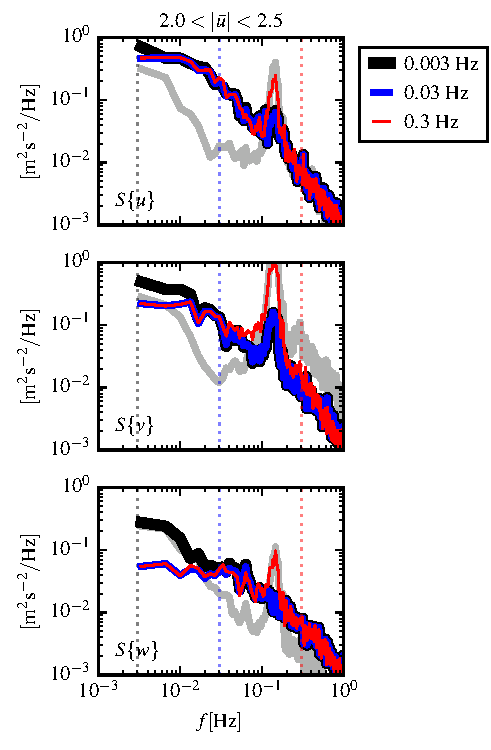
\includegraphics[width=\onewidth]{SpecFig04_filtering2}
  \caption{Motion-corrected velocity spectra, $\spec{\vec{u}}$, for a range of high-pass filter frequencies: $f_a= 0.3$ Hz (thin red), 0.03 Hz (blue), and 0.003 Hz (thick black). The vertical dashed lines indicate the filter frequency. The thick grey line is $\spec{\uhead}$ for $f_a=$ 0.003 Hz. The data are from the June 2014 TTM deployment when $2.0 < |\bar{u}| < 2.5\ \mathrm{ms^{-1}}$.
}
  \label{fig:filts}
\end{figure}

The choice of $f_a$ does influence the effectiveness of motion correction (Figure \ref{fig:filts}). When $f_a$ is too high (e.g., 0.3  Hz, red), the high-pass filter removes resolved motion from $\uhead$ that could be used to correct velocity measurements. In particular, notice that the amplitude of the 0.15 Hz peak---which is clearly the result of motion contamination (grey line)---is reduced significantly when we preserve more $\uhead$ information by reducing the high pass filter frequency to $f_a = 0.03$ Hz. Further reducing $f_a$ to $0.003$ Hz does not reduce the peak further, but does increase the amplitude of the spectra at low-frequency. This low-$f$ increase is the IMU-accelerometer's low-frequency bias drift (Figure \ref{fig:stnoise}) returning to contaminate the motion correction method.

Based on the above, we conclude that $f_a = 0.03$ Hz is a convenient `middle' frequency that reduces accelerometer bias-drift without destroying resolved motion of the TTM.  The same $f_a=0.03$ Hz filter was selected, based on a similar analysis, for the turbulence torpedo. The reader is likely to notice that the $0.15$ Hz peak is not completely removed by motion correction, especially for the $v$ component (Figure \ref{fig:filts}, middle panel). We will discuss this `persistent motion contamination' further in the following section.

Thus, we find that filter selection involves a trade-off between filtering out the bias drift noise at low-frequencies while not filtering out measured motion at high frequencies. In general, this will depend on the dynamics of the platform used to support the ADV, and the intensity of the turbulence being measured. When an independent measurement of $\ulow$ is available the cross-coherence with $\uacc$ can indicate a region of spectral overlap, and $f_a$ can be selected at the midpoint. Lacking a reliable estimate of $\ulow$,  the value of $f_a$ that produces the lowest $\tke$ estimates is likely the best. 

Additional details on motion correction---including a detailed accounting of the distinct coordinate systems of the IMU, ADV pressure case, and ADV head---can be found in \cite{Kilcher++2016}. Open-source Python tools for performing motion correction of ADV-IMU data---including scripts that write processed data in Matlab and tabulated formats---are available at \url{http://lkilcher.github.io/dolfyn/}.

\def\ue{\ensuremath{\vec{u}\earth}}

%%% Local Variables:
%%% mode: latex
%%% TeX-master: "Kilcher_etal_IMU-ADV"
%%% End:


\section{Results}
\label{sec:results}

\begin{figure}[t]
  \centering
  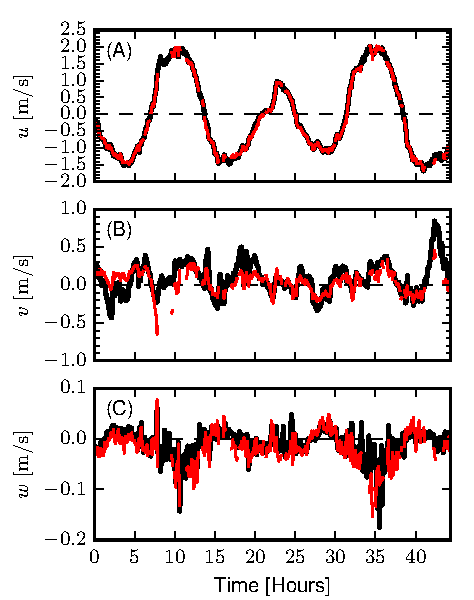
\includegraphics{TimeFig02}
  \caption{Time series of tidal velocity at Admiralty Head from TTM measurements (black), and an acoustic Doppler profiler (red). The profiler measurements--taken at the same depth as the ADV on the TTM---were contaminated by acoustic reflection from the strongback fin when it was inline with one of the profiler's beams. Note that the vertical scale on the three axes vary by more than an order of magnitude; the small ticks in A and B are equivalent to the ticks in C.}
  \label{fig:vel_time}
\end{figure}

\subsection{Mean velocity}

Figure \ref{fig:vel_time} shows a comparison of $\vec{\bar u}$ measured by an ADV-IMU mounted on a TTM, to that of an upward-looking acoustic Doppler profiler mounted on the TTM anchor. This shows excellent agreement between the ADV and Doppler profiler measurements of velocity. The $\bar u$, $\bar v$ and $\bar w$ components have a root-mean-square error of 0.05, 0.13 and 0.03 m/s, respectively.
%% Currently this is in the caption, but should it be in the text?
% The periods of missing profiler data occurred when the mooring interfered with one of the profiler's beams, as described in section \ref{sec:meas}. 
While it is important to note that their is some discrepancy between ADP and ADV measured velocities (especially in $\bar v$, which is most likely due to incomplete motion correction), the agreement between the magnitude and direction of these independent velocity measurements indicates that moored ADV-IMUs provide a reliable estimate of velocity in the Earth's reference frame.

\subsection{TTM spectra}

\begin{figure*}[t]
  \centering
  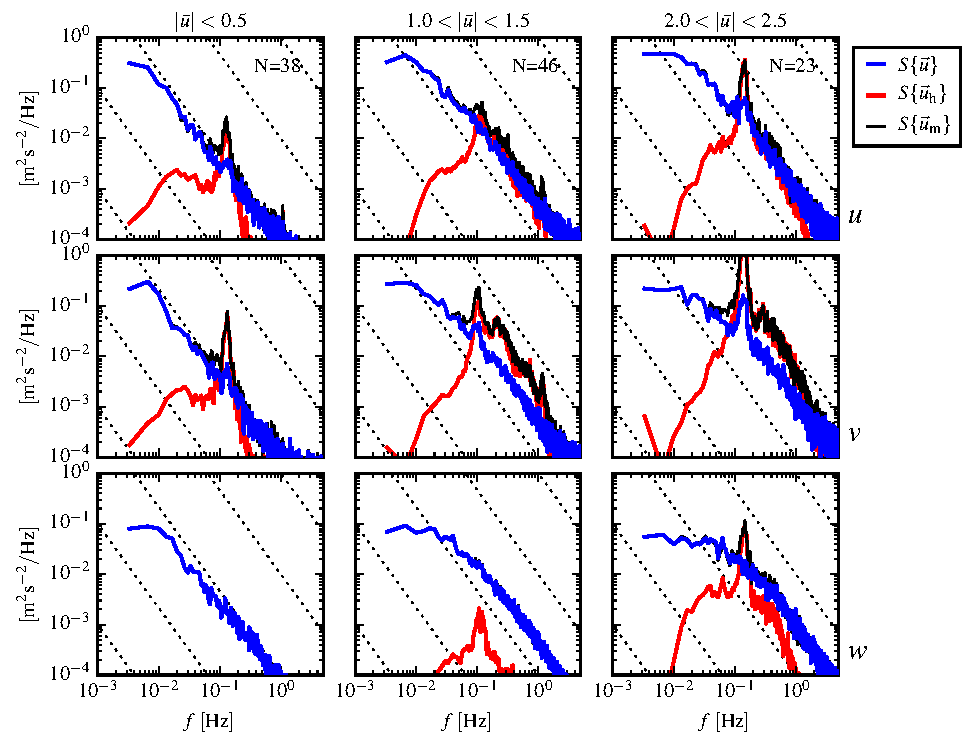
\includegraphics{SpecFig02_TTM02B-top}
  \caption{Turbulence spectra from the June 2014 TTM deployment. Each column is for a range of streamwise velocity magnitudes (indicated at top). The rows are for each component of velocity (indicated to the lower-right of the right column). The uncorrected spectra are in black and the corrected spectra are blue, and the spectra of ADV head motion, $\uhead$, is red (also indicated in the legend). The vertical red dotted line indicates the filter frequency applied to the IMU accelerometers when estimating $\uhead$; below this frequency $\spec{\uhead}$ is plotted as a dashed line.   Diagonal black dotted lines indicate a $f^{-5/3}$ slope. The number of spectral-ensembles, N, in each column is indicated in the top row.}
  \label{fig:spec:ttm}
\end{figure*}

As discussed in detail in Part 1 the mooring motion of the TTM, $\spec{\uhead}$, has a peak at 0.1 to 0.2 Hz from swaying of the mooring that is most likely driven by eddy-shedding from the spherical buoy (Figure \ref{fig:spec:ttm}, red lines). There is also higher-frequency broad-band motion that is associated with fluttering of the strongback fin around the mooring line. Both of these motions are especially energetic in the $v$-component spectra, because this is the direction in which the TTM mooring system is most unstable. As is expected from fluid-structure interaction theory the amplitude of these motions increases with increasing mean velocity \cite[]{Morison++1950}.

The mooring motion contaminates the uncorrected ADV-measurements of velocity, $\spec{\umeas}$, whenever the amplitude of the motion is similar to or greater than the amplitude of the turbulence. Fortunately, much of this motion can be removed using the IMU's motion signals as detailed in section \ref{sec:methods}. Lacking an independent measurement of turbulence velocity at this site, we interpret the agreement of these spectra with turbulence theory as evidence of the success of the method. In particular, at high-frequencies ($f>0.3$ Hz) for each mean-flow speed the spectra decay with a $f^{-5/3}$ slope and have equal amplitude across the velocity components. These results are consistent with Kolmogorov's (1941) theory of isotropic turbulence, and are consistent with other measurements of turbulence in energetic tidal channels from stationary platforms \cite[]{Kolmogorov1941c,Walter++2011,Thomson++2012,McMillan++2016}.

At low frequencies, the spectra tend to become roughly constant (especially at higher flow speeds), which is also consistent with previous works. Note here, that the very-low magnitude of $\spec{\uhead}$ at low frequencies is partially a result of filtering the IMU's accelerometer signal when calculating $\uacc$. The true low-frequency spectrum of ADV-head motion is unknown (indicated using a dashed line below $f_a$). A comparison of $\spec{\ue}$ measured by the TTM to that measured by the ADP---during the June 2012 deployment---are in agreement at low-frequencies (not shown). This suggests that the assumption that $\ulow=0$ at these frequencies, at this site, for this platform is justified---even if $\spec{\uhead}$ is not as low as indicated in Figure \ref{fig:spec:ttm}.

As successful as motion correction is, some of the motion contamination persists in $\spec{\ue}$. This is most notable in $\spec{v}$ at the highest flow speeds ($>2.0$ m/s): a peak at 0.15 Hz is an order of magnitude larger than a spectral fit to the other frequencies would indicate. This persistent motion contamination is evident to a lesser degree in $\spec{u}$ for $|u|>2$ m/s, and in $\spec{v}$ at lower flow speeds.  $\spec{w}$ appears to have no persistent motion contamination because the amplitude of the motion in this direction is much lower than for the other two components. For these measurements, $\spec{w_h}$ is so low that $w$-component motion correction is only necessary when $|u| > 2$ m/s.

The amplitude of the persistent motion contamination peaks in $\spec{v}$ at 0.15 Hz are a factor of 5 to 10 times smaller than the amplitude of the ADV head motion itself. This suggests the Microstrain IMU can be used to effectively correct for mooring motion at 0.15 Hz when the amplitude of that motion is less than 3 times the amplitude of the real turbulence spectrum. Where we have chosen a value of 3 as a conservative estimate of motion correction's effectiveness.

% Does this belong in the discussion?
This reveals an ancillary benefit of the IMU measurements: in addition to the primary benefit of correcting for mooring motion, they can also be used to identify and screen-out persistent motion contamination. For example, one of the most common uses of turbulence spectra is for the calculation of $\epsilon$ and $\tke$. For these purposes, based on the relative amplitudes of the 0.15 Hz peaks, we assume that persistent motion contamination is likely where $\spec{\uhead}/\spec{\ue} > 3$ and exclude these regions from spectral fits.

In the present case, for the $u$ and $w$ spectra, this criteria only excludes a narrow range of frequencies at the 0.15 Hz motion peak for some cases. This criteria is more restrictive of the $v$-component spectra at high frequencies for $\bar U > 1.0$ m/s, but this may be acceptable because the amplitude of the spectrum at these frequencies---i.e. in the isotropic inertial subrange---should be equal to that of $u$ and $w$ \cite[]{Kolmogorov1941c}.

Agreement of the $v$-component spectral amplitude with that of $u$ and $w$ at frequencies $>0.3$ Hz indicates that motion correction is effective at those frequencies even when $\spec{\uhead}/\spec{\ue} > 3$. This suggests that our screening threshold is excessively conservative at those frequencies, and that a more precise screening threshold is frequency dependent. For example, it might take into account the $~f^3$ character of the noise in $\spec{\uacc}$ (Figure \ref{fig:stationary_noise}). For the purposes of this work the $\spec{\uhead}/\spec{\ue} < 3$ threshold for spectral fits is sufficient, and detailed characterization of the IMU's motion- and frequency-dependent noise level is left for future work.

\subsection{StableMoor Spectra}

\begin{figure*}[th]
  \centering
  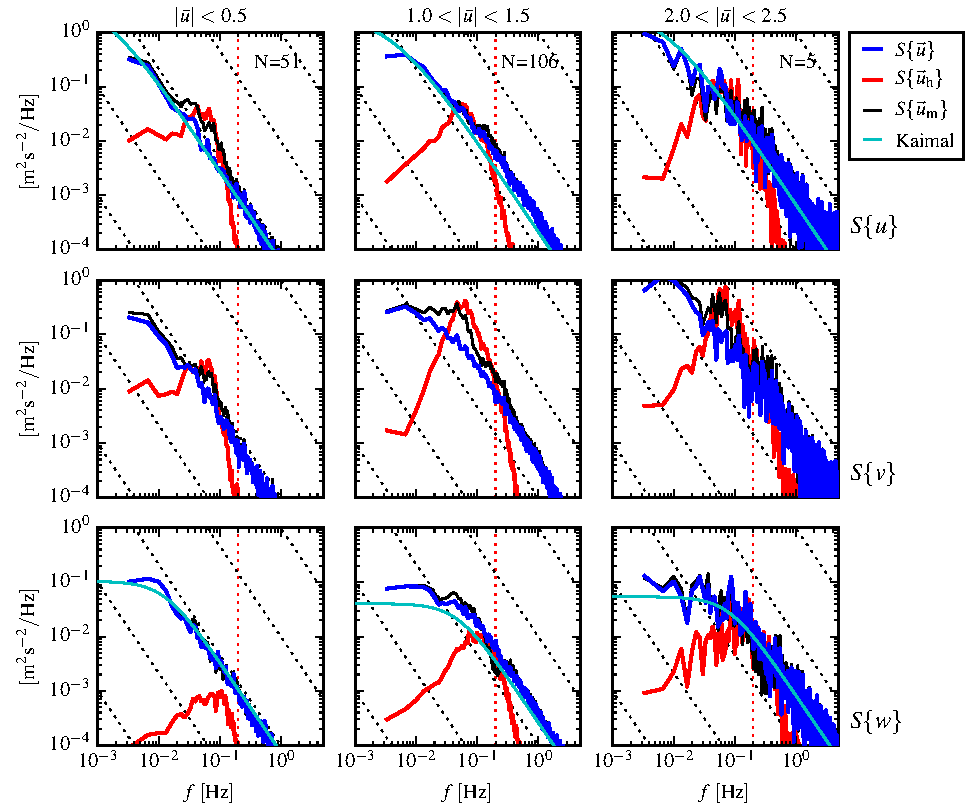
\includegraphics{SpecFig02_SMnose}
  \caption{Turbulence spectra from the StableMoor buoy. The axes-layout and annotations are identical to Figure \ref{fig:spec:ttm}, except that $\spec{\uhead}$ is plotted as a solid line at all frequencies because it is measured at all frequencies. }
  \label{fig:spec:sm}
\end{figure*}

The spectra of the stablemoor motion has a broader peak with a maximum amplitude that is approximately half the frequency of the TTM spectral peak (Figure \ref{fig:spec:sm}). The motion of this platform also does not have high-frequency `sub-peaks' or other high-frequency broad-banded excitation (Part 1).  These characteristics of the motion are most-likely due to the more massive and hydro-dynamically streamlined properties of the platform. 

Like the TTM, the motion-corrected spectra from the StableMoor are consistent with turbulence theory and previous observations. Most importantly, there is an improvement in the quality of the motion corrected spectra compared to the TTM. In particular the persistent motion contamination peaks appear to be completely removed. That is, this measurement system provides an accurate estimate of the turbulence spectra at this location from low frequencies to more than 1Hz---well into the inertial sub-range---for all three components of velocity.

Note that this level of accuracy can not be obtained without the independent estimate of $\ulow$. If we assume that $\ulow=0$ a similar plot to Figure \ref{fig:spec:sm} (not shown) reveals persistent motion-contamination peaks and troughs in the $u$- and $v$-spectra regardless of the choice of $f_a$. This indicates that the low-frequency motion of the StableMoor is below a threshold where the IMU's signal to noise ratio is high enough to resolve its motion. In other words, compared to the TTM, the StableMoor platform provides a more accurate measurement of turbulence when it includes an independent measure of $\ulow$ (here a bottom-tracking ADCP), but it does no better---and perhaps worse---when it doesn't.

\subsection{Torpedo spectra}

\begin{figure}[t]
  \centering
  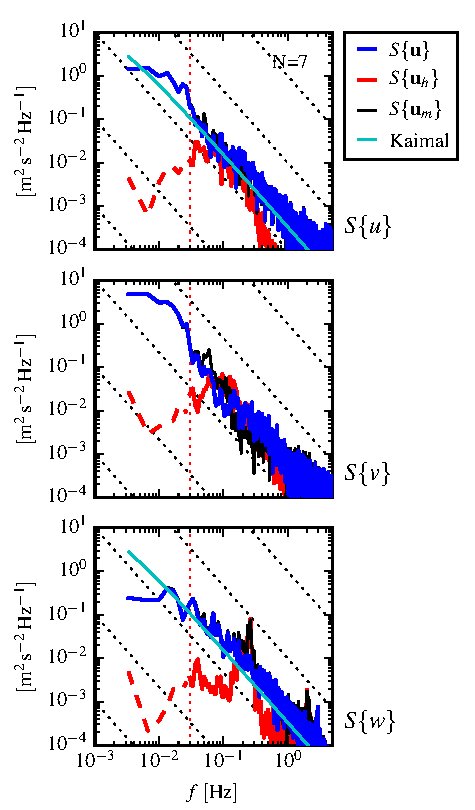
\includegraphics{SpecFig03_TTT}
  \caption{Turbulence spectra from the turbulence torpedo during a 35 minute period when the mean velocity was 1.3 m/s. Annotations and line colors are identical to Figure \ref{fig:spec:ttm}.}
  \label{fig:spec:torpedo}
\end{figure}

The $u$ and $v$ motion of the turbulence `torpedo' is broad-banded and the $w$ motion has a narrow peak at 0.3 Hz (Figure \ref{fig:spec:torpedo}). Because $\uhead$ is estimated using $f_a = 0.0333Hz$ and assuming $\ulow=0$ its spectra rolls-off quickly below $f_a$. A better estimate of $\ulow$ could be obtained by accounting for ship motion, but this has not been done here.

%Side note: even with the high-pass filtering the integration of the low-$f$ accelerometer noise appears as a `rebound' of the spectrum of $\uhead$ at the lowest frequencies.

Motion correction of the torpedo data appears to effectively remove a motion from $\spec{w}$ at 0.3Hz, and straightens out $\spec{v}$ between 0.04 and 0.6Hz. $\spec{u}$ is relatively unimproved by motion correction, apparently because the torpedo motion is smaller than the turbulence in this direction. At frequencies below $f_a$, $\spec{u}$ and $\spec{v}$ increase dramatically. This suggests that unresolved low-frequency motion of the torpedo is contaminating the velocity measurements at these frequencies. It may be possible to correct for some of this using a measurement of the ship's motion as a proxy for the torpedo's low-frequency motion, but this has not been done. Still, above $f_a$, the torpedo appears to provide a reliable estimate of spectral amplitude in the inertial subrange and can therefore be used to estimate $\epsilon$. Considering the simplicity of the platform it may be a useful option for quantifying this essential turbulence quantity in a variety of scenarios. If a GPS is positioned above it, it may be capable of providing even more.

\subsection{Cross-spectra}

\begin{figure*}[t]
  \centering
  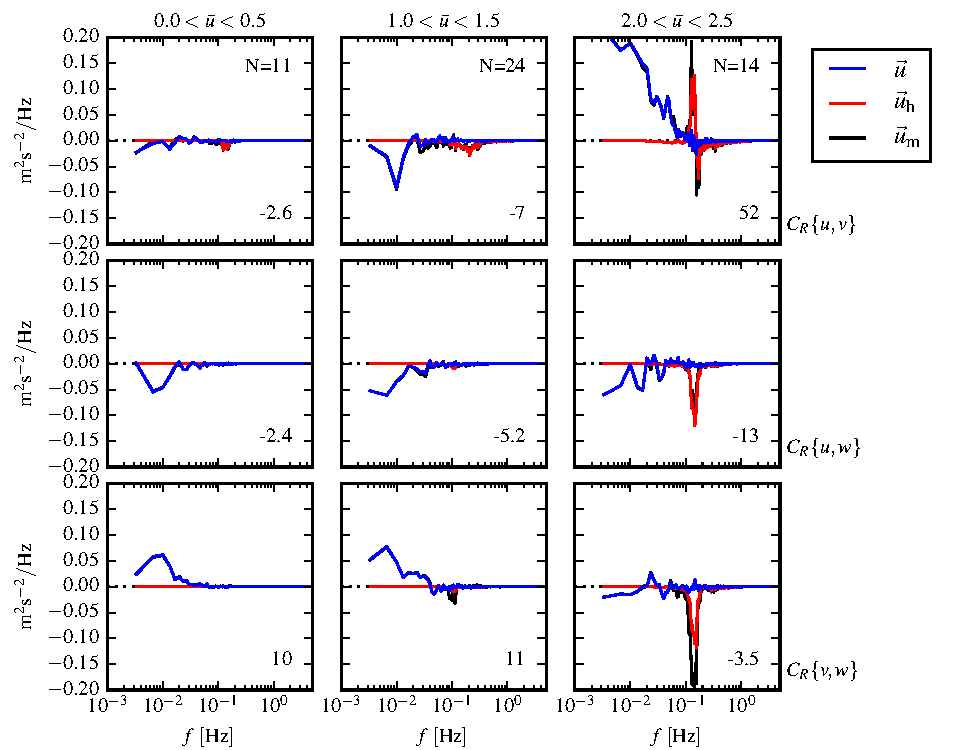
\includegraphics{StressSpec_TTM_03}
  \caption{The real part of the cross-spectral density between velocity components measured by the TTM. The upper-row is the $u$-$v$ cross-spectral density, the middle-row is the $u$-$w$ cross-spectral density, and the bottom-row is the $v$-$w$ cross-spectral density.  The columns are for different ranges of the stream-wise mean velocity magnitude (indicated above the top row). The blue line is the cross-spectrum between components of motion-corrected velocity, the red line is the cross-spectrum between components of head-motion, and the black line is the cross-spectrum between components of uncorrected velocity. The light-blue shading indicates one standard deviation of the $C$ for the motion corrected cross-spectral density. N is the number of spectral ensembles in each column. The number in the lower right corner of each panel is the motion-corrected Reynold's stress (integral of the blue line) in units of 1e-4 $\mathrm{m^2s^{-2}}$.}
  \label{fig:cspec:ttm}
\end{figure*}

Inspection of cross-spectra from TTM measurements demonstrates that motion correction can reduce motion contamination to produce reliable estimates of velocity cross-spectra (Figure \ref{fig:cspec:ttm}). At low flow speeds (left column), cross-spectra between components of $\uhead$ (i.e. between components of head-motion, red) are small compared to correlated velocities. As the velocity magnitude increases (center, and right columns), the swaying motion of the TTM at 0.15 Hz appears as a peak in the amplitude of the cross-spectra of $\uhead$ and $\umeas$ (black) for all three components of cross-spectra (rows). Fortunately, motion correction reduces the amplitude of this peak dramatically so that $C\{\ue\}$ (blue) is small at 0.15 Hz compared to lower frequencies. Furthermore, the fact that the standard deviation of $C\{\ue\}$ is also relatively small at 0.15 Hz suggests that motion correction is effective for each spectral window, not just in their mean.

These results indicate that motion-corrected TTM velocity measurements can be used to obtain reliable estimates of turbulence Reynold's stresses, which are the integral of the cross-spectra. Without motion correction, Reynold's stress estimates would be contaminated by the large peaks in the cross-spectra that are due to the swaying and fluttering motion of the TTM vane.

A similar investigation of StableMoor cross-spectra (not shown) indicates that cross-spectral motion contamination is much lower amplitude than for the TTM. The low-frequency ($<0.3$ Hz) `swimming' motion of that platform produces minimal cross-spectral signal, and the relative large-mass of the platform minimizes the kinds of higher-frequency swaying/fluttering that creates large values of cross-spectral head-motion. Thus, the StableMoor platform also produces reliable estimates of Reynold's stresses, which are presumed to be improved by motion correction.

%\section{Other stuff}




%%% Local Variables:
%%% mode: latex
%%% TeX-master: "Kilcher_etal_IMU-ADV"
%%% End:



\section{Discussion}

\begin{figure*}[t]
  \centering
  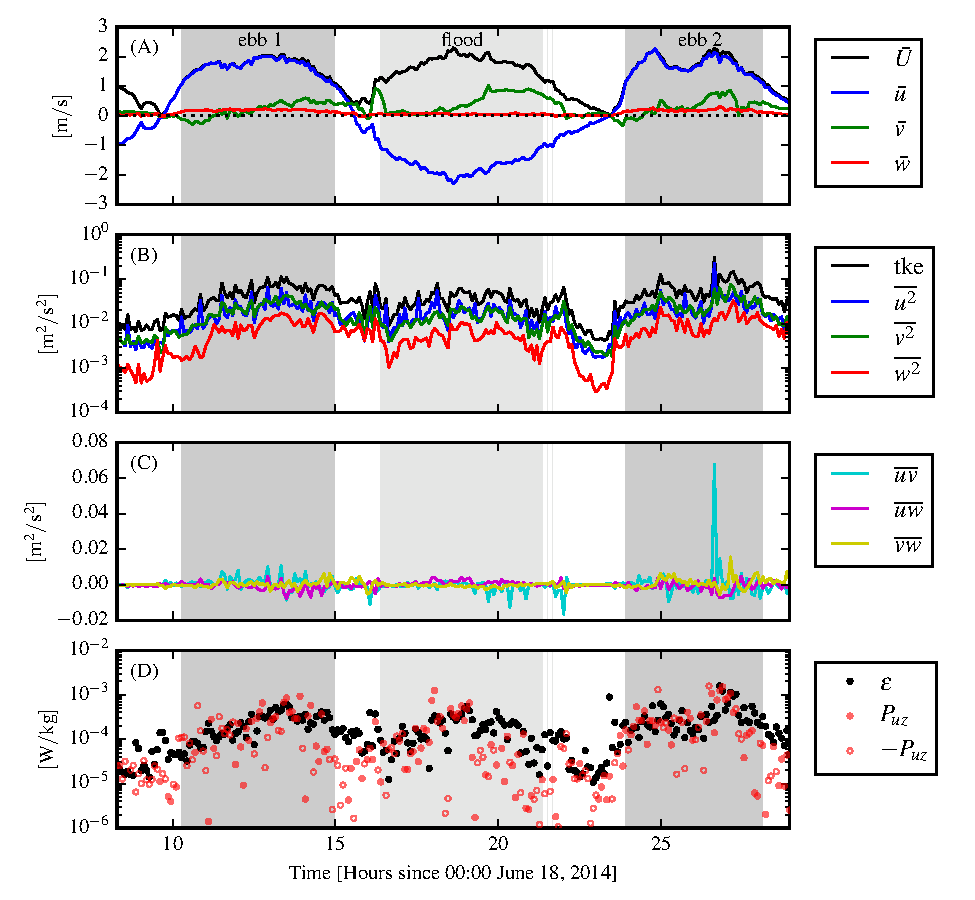
\includegraphics{TurbTime_TTM_01}
  \caption{Time-series of mean velocities (A), turbulence energy and its components (B), Reynold's stresses (C), and turbulence dissipation rate (D) measured by the TTM during the June, 2014 deployment. Shading indicates periods of ebb ($\bar{u}>1.0$, grey), and flood ($\bar{u}<-1.0$, lighter grey).}
  \label{fig:turbtime:ttm}
\end{figure*}

The beginning of the previous section presented a comparison of $\vec{\bar{u}}$ measured by a TTM-mounted ADV, to measurements from a co-located ADP. This demonstrated that the IMU provides a reliable estimate of the ADV's orientation and that this can be utilized to estimate mean velocity in the earth's reference frame. Turbulence velocity estimates from the same ADP are also in agreement with low-frequency TTM turbulence estimates (not shown), but the ADP does not resolve turbulence at the scales where motion contamination is strongest (0.1 to 1.0 Hz).

Ideally, moored motion-corrected turbulence velocity measurements would be validated against simultaneous independent validated measurements of turbulence velocity at the same scales, exact time and exact location. Accomplishing this, however, involves significant technical challenges not easily overcome---most notably the difficulty of measuring turbulence at the same point as the moving ADV. A slightly less ideal but much more realistic confirmation of the methodology might involve comparing the statistics of moored turbulence measurements to that from a nearby fixed platform, or a fixed platform placed at the same location at a different time \citep[e.g. the `TTT' platform described in][]{Thomson++2012}. Unfortunately, to our knowledge, these measurements have not yet been made.

Lacking a relevant, fixed, independent turbulence measurement to compare to it is instructive to demonstrate the degree to which the moored measurements are consistent with turbulence theory and other turbulence measurements in similar flow environments. The previous section showed that the shape of the turbulence velocity spectra from moored ADVs is consistent with Kolmogorov's theory of locally isotropic turbulence, which has been observed consistently in turbulence measurements for decades \citep[]{Kolmogorov1941c,Grant++1962,McMillan++2016}. In particular, we observed an isotropic subrange---an $f^{-5/3}$ spectral slope, and equal amplitude spectra between components---that is driven by anisotropic turbulence at longer time-scales (Figures \ref{fig:spec:ttm}, \ref{fig:spec:sm}, \ref{fig:spec:torpedo}). This is interpreted as the first indication that the measurement systems presented are capable of accurately resolving turbulence. The degree to which uncorrected spectra were corrected toward this theoretical and observationally confirmed shape is interpreted as a measure of the improvement of the spectral estimates by motion correction.

Figure \ref{fig:turbtime:ttm} presents a time-series of the mean velocity (A) and several turbulence statistics that were measured during the June 2014 TTM deployment. This figure shows the evolution of the flow through Admiralty Inlet during 1.5 tidal cycles. The $\tke$ (B), Reynold's stresses (C), dissipation and one component of turbulence production (D) grow and strengthen with ebb or flood, then subside during slack tide.  This component of turbulence production is:
\begin{align}
  \produz = \frac{\partial \bar{u}}{\partial z}\uw \qquad .
\end{align}
Where $\partial \bar{u}/\partial z$ is computed from the two ADV's on the TTM. The highest values of $\epsilon$ and $\produz$ occur at the peak of the ebb or flood, which is in agreement with other measurements in tidal channels. The agreement of the magnitude of $\produz$ with $\epsilon$ at those times suggests a local production-dissipation balance that is often observed in tidally forced channels \citep[]{Trowbridge++1999,Stacey++1999,McMillan++2016}. At other times the value of $\produz$ is insufficient to balance $\epsilon$ or is negative.

\begin{figure}[t]
  \centering
  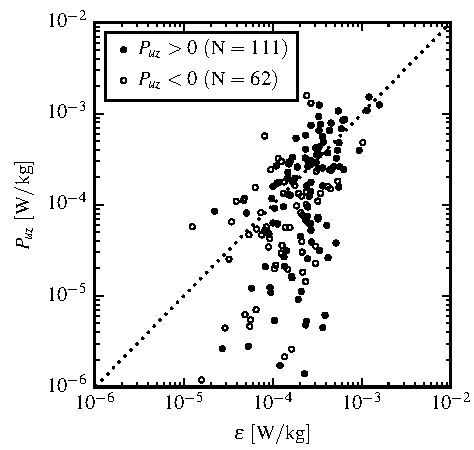
\includegraphics{EpsVProd01}
  \caption{$\produz$ vs. $\epsilon$ during the June 2014 TTM deployment for values of $|u|>1$ m/s. Values of `negative' production are indicated as open circles. }
  \label{fig:prodVeps}
\end{figure}

Inspection of the negative $\produz$ values reveals that most of them are due to a reversed sign of $\uw$ rather than a reversed sign of $\partial u / \partial z$ (i.e. when compared to the sign of $u$). This suggests that uncertainty in $\uw$ may be contributing to discrepancies between $\produz$ and $\epsilon$. It is also possible that other terms of the $\tke$ equation are important, such as other components of production, advection terms, or turbulent transport terms.

Figure \ref{fig:prodVeps} compares individual values of $\produz$ with $\epsilon$ directly. Given the assumptions implicit in this comparison, and the discussion above, the agreement between $\produz$ and $\epsilon$ is an encouraging result that suggests the turbulent boundary reaches the depth of these measurements (10 m) during the highest flow speeds. This result is further supported by a comparison of $\bar{U}$ with $\epsilon$ (Figure \ref{fig:epsVu}). Here we see a $\epsilon \propto \bar{U}^3$ dependence that is again suggestive of bottom boundary layer physics \citep[]{Trowbridge1992,Nash++2009}. At lower flow speeds, $\epsilon$ deviates from this relationship, which suggests that the boundary layer is no longer the dominant physical process at the depth of these measurements.


\begin{figure*}[t]
  \centering
  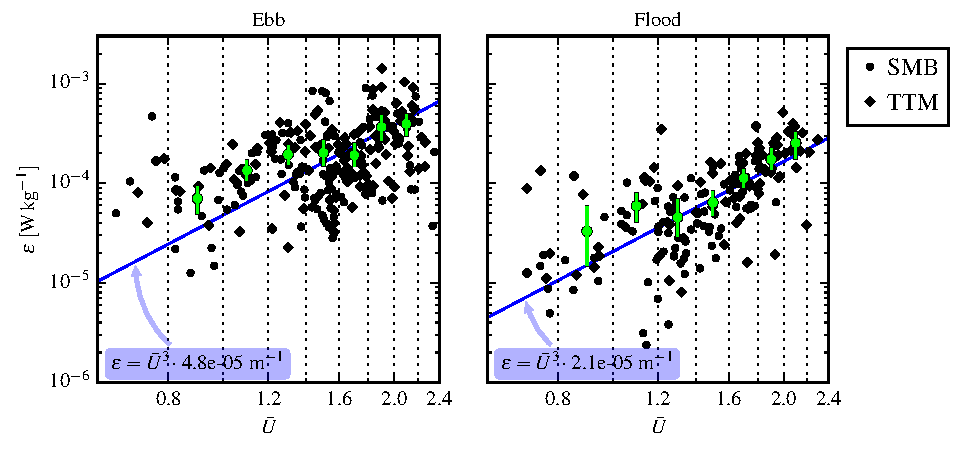
\includegraphics{EpsVU_03}
  \caption{A log-log plot of $\epsilon$ versus $\bar{U}$ for the June 2014 TTM (diamonds) and May 2015 StableMoor (dots) deployments, during ebb (left) and flood (right). Black points are 5 minute averages.  Green dots are mean values within speed bins of 0.2 m s$^{-1}$ width that have at least 10 points (50 minutes of data); their vertical bars are 95\% bootstrap confidence intervals. The blue line shows a $U^3$ slope, where the proportionality constant (blue box) is calculated by taking the log-space mean of $\epsilon/U^3$. }
  \label{fig:epsVu}
\end{figure*}



%%% Local Variables:
%%% mode: latex
%%% TeX-master: "Kilcher_etal_IMU-ADV"
%%% End:



\section{Conclusion}
\label{sec:conclusion}
 
This work presents a methodology for measuring turbulence from moored ADV-IMUs and demonstrates that motion correction reduces mooring motion-contamination. Comparison of spectra of ADV head motion, $\spec{\uhead}$, to that of motion-corrected, $\spec{\ue}$, and uncorrected spectra, $\spec{\umeas}$, reveals that motion correction improves spectral estimates of moored ADV measurements. In particular, we found that motion-corrected spectra have spectral shapes that are similar to previous measurements of tidal-channel turbulence and have a $f^{-5/3}$ spectral slope at high frequencies. This finding suggests that the motion-corrected spectra resolve the inertial subrange predicted by Kolmogorov's theory of locally isotropic turbulence.

Motion correction reduces motion contamination for all platforms we presented but it does not necessarily remove it completely. This outcome seems to depend on the relative amplitude of platform motion compared to the underlying turbulence being measured. The most notable example of this is from the TTM, which has a large ``swaying" peak at 0.1 Hz. Where this peak is very large---especially in the $v$ component---it is not reduced to a level that is consistent with earlier measurements of tidal-channel turbulence---i.e., there is no smooth roll-off between the low-frequency energy-containing scales and the $f^{-5/3}$ inertial subrange.

This inconsistency indicates that turbulence measurements from moored, motion-corrected IMU ADVs must be interpreted with care. An inspection of spectra presented here suggests that excluding spectral regions where $\spec{\uhead} / \spec{\ue} > 3$ removes persistent-motion contamination peaks while still preserving spectral regions where motion correction is effective. Using this criteria, it is then possible to produce spectral fits that exclude persistent-motion contamination, and provide reliable estimates of turbulence quantities of interest (e.g., $\epsilon$ and $\tke$).

We've also shown that motion correction reduces motion contamination in cross spectra. This finding is important because it suggests that moored IMU-ADV measurements may be used to produce reliable estimates of Reynolds stresses. We utilized these stress estimates and vertical shear estimates, both from the TTM, to estimate $\produz$. 

Finally, we have shown that $\epsilon$ estimates based on motion-corrected spectra scale with the $U^3$, and balance $P_{uz}$ estimates during ebb and flood. Together, these results indicate that bottom boundary layer physics are a dominant process at this site, and that the boundary layer reaches the height of the IMU ADVs (10 m) during ebb and flood. The degree of agreement between $\produz$ and $\epsilon$ also serves as an indicator of the self-consistency of moored IMU-ADV turbulence measurements. 

%%% Local Variables:
%%% mode: latex
%%% TeX-master: "Kilcher_etal_IMU-ADV"
%%% End:


\acknowledgments

Many thanks to Joe Talbert, Alex DeKlerk, Captain Andy Reay-Ellers,  Jennifer Rinker, Maricarmen Guerra, and Eric Nelson in assisting with data collection. The authors are also grateful to James VanZwieten, Matthew Egeland and Marshall Richmond for discussion on the details of this work.

This work was supported by the U.S. Department of Energy under Contract No. DE-AC36-08GO28308 with the National Renewable Energy Laboratory. Funding for the work was provided by the DOE Office of Energy Efficiency and Renewable Energy, Wind and Water Power Technologies Office. 

The U.S. Government retains and the publisher, by accepting the article for publication, acknowledges that the U.S. Government retains a nonexclusive, paid-up, irrevocable, worldwide license to publish or reproduce the published form of this work, or allow others to do so, for U.S. Government purposes.

\clearpage %REMOVE_FOR_SUBMIT

%%%%%%%%%%%%%%%%%
%APPENDIXES
%%%%%%%%%%%%%%%%%
\appendix

\section{Comparing StableMoor $\ulow$ to IMU $\uhead$}
\label{apdx:ulow}

\def\ubt{\ensuremath{u_\mathrm{BT}}}

\begin{figure}[t]
  \centering
  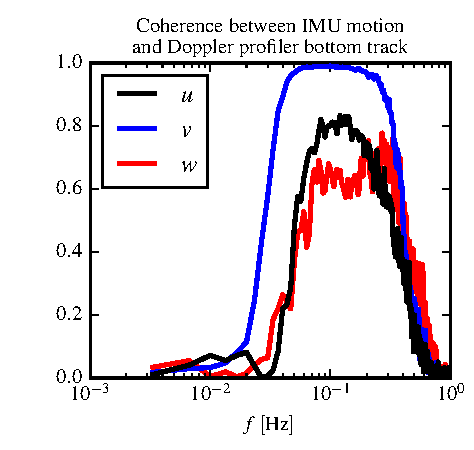
\includegraphics{BT_IMU_Coherence02}
  \caption{Coherence between IMU-measured motion of StableMoor buoy and ADP bottom track velocity for $1.0<\bar{U}<1.5$. The horizontal dotted line indicates the 95\% confidence level for the 102 spectral windows in this estimate.}
  \label{fig:SM_coh}
\end{figure}
To better understand the IMU's signal-to-noise ratio, we compare the motion of the StableMoor buoy from the ADP bottom track measurements, $\ubt$, to the IMU's estimates of ADP motion. To do this, we compute the IMU's estimate of ADP motion using equation \eqref{eqn:uhead}, and replacing $\ell^{*}$ with the vector that points from the IMU to the ADP head. We then linearly interpolate the ADP measurements onto the times of the ADV-IMU measurements.

The coherence between these two signals is high and statistically significant over 1.5 decades---from 0.03 to 0.8 Hz \cite[][]{Priestley1981}. The $v$ component has the highest coherence, 98\%, because this is the direction that has the most motion. Therefore, these estimates have a higher signal-to-noise ratio.  The $u$ and $w$ components have a slightly lower coherence, 80\% and 65\%, respectively, which indicates the ``convolved'' signal-to-noise ratio of these measurements.

On the low-frequency side, our interpretation is that the signal-to-noise ratio of the IMU increases dramatically below 0.03 Hz, resulting in low coherence. On the high-frequency side, Doppler noise in the ADP measurements contaminates its estimates of motion, causing the decrease in coherence at 0.8 Hz. A comparison of the phase between these signals shows that there is no lag between the measurements (not shown).


These results help to inform the selection of zero-lag filters used to estimate $\ulow$ from $\ubt$. In particular, by selecting 0.2 Hz, we target the middle of the coherence peak between the two measurements. Furthermore, the rapid decrease in coherence below 0.03 Hz provides an objective measurement of the performance of the frequency at which IMU measured velocity becomes unreliable in the flow conditions we observed. 



%%% Local Variables:
%%% mode: latex
%%% TeX-master: "Kilcher_etal_IMU-ADV"
%%% End:


%%%%%%%%%%%%%%%%%
%REFERENCES
%%%%%%%%%%%%%%%%%

\bibliographystyle{ametsoc2014}
\bibliography{thisbib}


\end{document}
